\documentclass[12pt,a4paper]{article}
\usepackage[utf8]{inputenc}
\usepackage[francais]{babel}
\usepackage[T1]{fontenc}
\usepackage{amsmath}
\usepackage{amsfonts}
\usepackage{amssymb}
\usepackage{float}
\usepackage[left=2cm,right=2cm,top=2cm,bottom=2cm]{geometry}
\usepackage{graphicx}
\usepackage{tabularx}
\usepackage{array}

\newcommand{\HRule}{\rule{\linewidth}{0.5mm}}

\begin{document}
%%% Page de garde %%%
\begin{titlepage}
\begin{center}


\includegraphics[width=0.3\textwidth]{images/universite_bordeaux_logo.png}\\[1cm]    


\textsc{\Large Projet de Fin d'Etude}\\[0.5cm]
\textsc{\Large Master 2 Systèmes mobiles autonomes communicants}\\[0.5cm]

\vspace{30pt}
% Title
\HRule \\[0.4cm]
{ \huge \bfseries Rapport - Cas d'utilisation\\[0.7cm]
OpenRPAS \\[0.5cm]
Un simulateur ouvert
de système de drone}\\[0.4cm]

\HRule \\[1.5cm]

% Author and supervisor
\begin{minipage}{0.4\textwidth}
\begin{flushleft} \large
\textbf{Auteurs :}\\
Kinda \textsc{Al Chahid}\\
Alexandre \textsc{BROUSTE}\\
Salah Eddine  \textsc{Bouyahmed}\\
Ali  \textsc{ZAMOUCHE}\\
Youssef \textsc{Dichkour}\\
Imane \textsc{Zerouali}
\end{flushleft}
\end{minipage}
\begin{minipage}{0.4\textwidth}
\begin{flushright} \large
\textbf{Responsable :} \\
Serge \textsc{Chaumette}\\
\end{flushright}
\end{minipage}

\vfill

% Bottom of the page
{\large \today}

\end{center}

\end{titlepage}




\section{Cas d'utilisation}

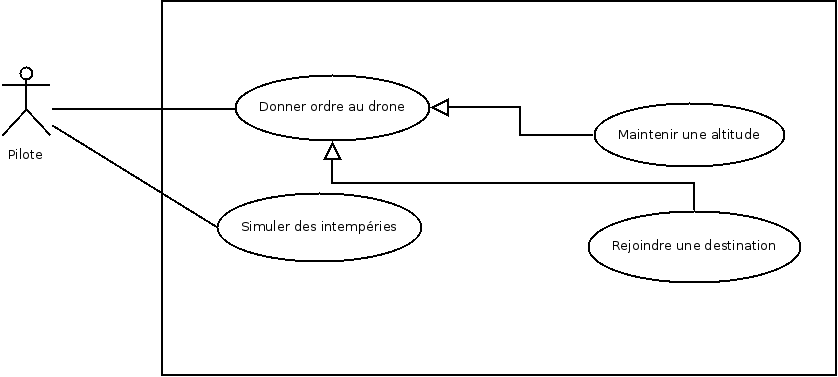
\includegraphics[width=1\textwidth]{images/Diagramme1.png}\\[1cm]    



\section{Scénario}
Ce projet comporte 3 parties : un simulateur de drone, une base et un bus.\\


\underline{Scénario nominal}

L'utilisateur envoie une destination et une altitude a la base.
La base envoie l'ordre au bus.
Le bus transfert cet ordre au drone.
Le drone ajuste sa position et son altitude en fonction des données reçues par les capteurs.
Le drone envoie en permanence touts les données reçues par les capteurs a la base en passant par le bus.
La base affiche pour l'utilisateur ces données.\\

\underline{Scénario alternatif}

L'utilisateur peut simuler des intempéries auquel cas le drone doit adapter sa position et son attitude.




\end{document}
